\appendix
% elsarticle 的 \appendix 不重置 figure 计数器，正文那张框架图已经把它推到 1，
% 附录图因此会被编成 C.2/C.3，读者会去找并不存在的 C.1。
\setcounter{figure}{0}

\section{Supporting statistics}
\label{app:significance}

Sec.~\ref{sec:setup} fixes the confirmatory family and states the correction policy. This
appendix lists the individual comparisons behind that family, so that none of the verdicts
has to be taken on trust or reconstructed from prose.
Table~\ref{tab:appendix-signif-a} \emph{is} the confirmatory family: FOLoRA against each
baseline of Table~\ref{tab:main}, on average accuracy, with the uncorrected and the
Holm-corrected $p$ side by side. Table~\ref{tab:appendix-signif-b} collects the
comparisons the body quotes in prose but no other table covers --- the same-$\lambda$
Fisher-weighting contrast, the $k{=}16$ sweep, and the two orthogonality strengths of
O-LoRA --- either because they are not against the main configuration or because their
seed budgets differ from it. The two are kept apart rather than merged into one table
because their correction conventions differ. Table~\ref{tab:appendix-signif-a} is the
confirmatory family and reports corrected $p$-values throughout.
Table~\ref{tab:appendix-signif-b} is exploratory: it is quoted uncorrected, with the single
exception its caption states --- the two O-LoRA orthogonality points form a two-member
family per benchmark that the body quotes \emph{with} its within-family correction, so that
block's $p_{\mathrm{Holm}}$ column is filled in and the remaining rows leave it blank.
A corrected $p$ from one family should not be read against a corrected $p$ from another.

Three conventions hold throughout. $n$ is always the number of seeds
\emph{common} to the two arms of that row, never a shared budget, so rows with different
$n$ do not have the same power and their $p$-values should not be compared as if they did.
$\Delta$ is FOLoRA minus the comparison, in accuracy points, so positive favours FOLoRA;
on the gap metric reported in the body the sign convention is the opposite, which is one
reason the two are tabulated separately. And a row whose $n$ is below two carries no test
at all: it is listed with $p$ given as \emph{n/a} rather than dropped, because the reason
a point cannot support a claim is part of the record.

% Generated by scripts/make_paper_tables.py; do not edit by hand.
\begin{table}[tbp]
\centering\small
\caption{The confirmatory family of Sec.~\ref{sec:setup}: FOLoRA against
each baseline of Table~\ref{tab:main} on average accuracy, with both the
uncorrected $p$ and the Holm--Bonferroni corrected $p_{\mathrm{Holm}}$ that
the paper's verdicts rest on. Conventions are stated above; the exploratory
comparisons are in Table~\ref{tab:appendix-signif-b}.}
\label{tab:appendix-signif-a}
\setlength{\tabcolsep}{4pt}
\begin{tabular}{@{}llcccc@{}}
\toprule
Benchmark & Comparison & $n$ & $\Delta$ & $p$ & $p_{\mathrm{Holm}}$ \\
\midrule
\multicolumn{6}{@{}l}{\emph{Confirmatory family: Table~\ref{tab:main}, average accuracy}} \\
CIFAR-100 & Seq-LoRA & 10 & +8.56 & 0.0000 & 0.0000 \\
CIFAR-100 & EWC-LoRA (lam=100) & 10 & +0.65 & 0.0734 & 0.2934 \\
CIFAR-100 & EWC-LoRA (lam=300) & 10 & -0.14 & 0.6440 & 0.9921 \\
CIFAR-100 & EWC-LoRA (lam=1000) & 10 & +0.21 & 0.4961 & 0.9921 \\
CIFAR-100 & EWC-LoRA (lam=3000) & 10 & +0.47 & 0.2507 & 0.7521 \\
CIFAR-100 & O-LoRA & 10 & +12.92 & 0.0000 & 0.0000 \\
CIFAR-100 & L2P & 5 & +4.67 & 0.0002 & 0.0013 \\
CIFAR-100 & CODA-Prompt & 5 & +3.61 & 0.0016 & 0.0080 \\
CIFAR-100 & InfLoRA & 5 & +5.37 & 0.0002 & 0.0014 \\
ImageNet-R & Seq-LoRA & 5 & +10.34 & 0.0002 & 0.0011 \\
ImageNet-R & EWC-LoRA (lam=100) & 10 & +2.85 & 0.0002 & 0.0011 \\
ImageNet-R & EWC-LoRA (lam=300) & 10 & +0.05 & 0.9010 & 1.0000 \\
ImageNet-R & EWC-LoRA (lam=1000) & 10 & +0.04 & 0.9235 & 1.0000 \\
ImageNet-R & O-LoRA & 5 & +13.20 & 0.0000 & 0.0000 \\
ImageNet-R & L2P & 5 & +7.45 & 0.0000 & 0.0000 \\
ImageNet-R & CODA-Prompt & 3 & +7.58 & 0.0022 & 0.0066 \\
ImageNet-R & InfLoRA & 3 & +7.96 & 0.0011 & 0.0046 \\
\bottomrule
\end{tabular}
\end{table}


% Generated by scripts/make_paper_tables.py; do not edit by hand.
\begin{table}[tbp]
\centering\small
\caption{The remaining comparisons the body quotes in prose, which no
other table covers: variants of the main configuration and of one
baseline, on both benchmarks. These are \emph{exploratory} --- chosen
after seeing the results --- so $p$ is uncorrected and each entry's family
is stated where its number is used in Sec.~\ref{sec:main_results}. The
O-LoRA training-time block is the one exception: the body quotes those
numbers with their within-family correction, given in the last column.
Columns and conventions are those of Table~\ref{tab:appendix-signif-a}.}
\label{tab:appendix-signif-b}
\setlength{\tabcolsep}{4pt}
\begin{tabular}{@{}llcccc@{}}
\toprule
Benchmark & Comparison & $n$ & $\Delta$ & $p$ & $p_{\mathrm{Holm}}$ \\
\midrule
\multicolumn{6}{@{}l}{\emph{Exploratory (uncorrected $p$)}} \\
\multicolumn{6}{@{}l}{\emph{~~Fisher-weighted against equal-weighted, same $\lambda$}} \\
CIFAR-100 & $\lambda{=}1$ & 5 & +3.83 & 0.0120 & --- \\
CIFAR-100 & $\lambda{=}3$ & 10 & +4.19 & 0.0000 & --- \\
CIFAR-100 & $\lambda{=}10$ & 5 & +0.38 & 0.6865 & --- \\
CIFAR-100 & $\lambda{=}30$ & 5 & -2.79 & 0.0039 & --- \\
\multicolumn{6}{@{}l}{\emph{~~$k{=}16$ protected directions against the $k{=}64$ main configuration}} \\
CIFAR-100 & $\lambda{=}3$ & 5 & +0.17 & 0.7487 & --- \\
CIFAR-100 & $\lambda{=}10$ & 5 & +0.41 & 0.3832 & --- \\
CIFAR-100 & $\lambda{=}30$ & 1 & +0.36 & n/a & --- \\
CIFAR-100 & $\lambda{=}100$ & 3 & +3.02 & 0.1489 & --- \\
CIFAR-100 & $\lambda{=}300$ & 10 & +4.25 & 0.0000 & --- \\
CIFAR-100 & $\lambda{=}1000$ & 3 & +4.52 & 0.0561 & --- \\
\multicolumn{6}{@{}l}{\emph{~~O-LoRA orthogonality strength ($p_{\mathrm{Holm}}$: two-member family)}} \\
CIFAR-100 & $\lambda_1{=}0.1$ & 5 & +7.10 & 0.0000 & 0.0001 \\
CIFAR-100 & $\lambda_1{=}1$ & 5 & +5.60 & 0.0002 & 0.0002 \\
ImageNet-R & $\lambda_1{=}0.1$ & 3 & +10.59 & 0.0172 & 0.0344 \\
ImageNet-R & $\lambda_1{=}1$ & 3 & +5.74 & 0.0174 & 0.0344 \\
\bottomrule
\end{tabular}
\end{table}


\section{The probe behind Sec.~\ref{sec:tightness}}
\label{app:tightness}

Sec.~\ref{sec:tightness} states the conclusion of the bound-tightness probe and the main
text uses only that conclusion. This appendix carries the protocol and the individual
measurements, so that the claim can be checked rather than taken on trust.

\paragraph{Protocol}
All numbers below come from an in-training probe that, at each task boundary of a 20-task
run, fits the expansion of the accumulated past-task loss along the \emph{realized}
adapter displacement,
$\Delta\mathcal{L}(\alpha\,\delta\theta)=a\alpha+b\alpha^{2}+c\alpha^{3}+\mathcal{O}(\alpha^{4})$,
over $\alpha\in[0,1.5]$. Measuring the nonlinearity along the realized displacement, rather
than bounding $L_3$, is what makes the remainder checkable at all: $L_3$ is not recoverable
from any stored checkpoint, whereas $a$, $b$ and $c$ are. We report $a$ and $c$ as ratios
to $|b|$, so that ``is this correction small?'' is read directly off the number. The probe
run is FOLoRA at $\lambda{=}10$, $k{=}16$, seed~0 on Split CIFAR-100, giving 19 usable
boundaries. It is a single configuration, and we do not have the seed spread needed to say
how much of what follows is run-to-run variation; the numbers should be read as one
operating point, not as a distribution over the method.

\paragraph{(i) The remainder is not negligible}
The ratio $|c|/|b|$ has median $0.163$, minimum $0.010$ and maximum $2.46$, with $5$ of the
$19$ boundaries above $0.30$. Under the decision rule frozen before these numbers were
computed (median $\le 0.10$: keep the negligibility claim; $0.10<\text{median}\le 0.30$:
weaken it; $>0.30$: drop it), this lands in the middle band, and the honest reading is the
one the frozen rule prescribes: the cubic term is \emph{of the same order as, but does not
dominate}, the quadratic term. The tail is the part that matters --- at the worst boundary
the quantity the bound calls a remainder is $2.5\times$ the quantity FOLoRA minimizes.

\paragraph{(ii) The stationarity residual is not small either}
The ratio $|a|/|b|$ has median $0.99$ and maximum $23.1$.
Assumption~\ref{ass:stationary} is stated for the \emph{unregularized} loss, so at a
regularized endpoint the residual is $-\lambda\nabla\Omega$, and
Remark~\ref{rem:regularized} argued that it should vanish proportionally to the
displacement. It does not vanish fast enough to be dropped: at the realized displacement
the linear term is comparable to the quadratic one, so the ``quadratic plus corrections''
reading of the expansion is not numerically available at this $\lambda$.

\paragraph{(iii) The Fisher estimate is not a calibrated surrogate for the curvature}
The ratio between the term the bound prescribes, $\frac12\delta\theta^{\!\top}\bar{F}\delta\theta$,
and the quadratic coefficient $b$ fitted from the same measurement has median
$2.8\times10^{-5}$: the finite-sample, rank-$k$, block-diagonal estimate of $F_\tau$
underestimates the measured curvature of the past loss along the realized displacement by
four to five orders of magnitude.
It is worth being precise about what this does and does not say. It does \emph{not}
contradict Theorem~\ref{thm:forgetting}, which is stated for the exact $F_\tau$; it says
that Assumption~\ref{ass:fisher} is far from innocuous at this operating point, which is
precisely the regime the empirical-Fisher literature warns about~\cite{kunstner2019limitations}.
It is also, in part, the intended behaviour seen from the other side: the displacement is
close to orthogonal to the top-$k$ Fisher subspace \emph{by construction}, since suppressing
that alignment is what the penalty does, so the Fisher-weighted quadratic form is small
along it. Both readings agree on the operative point: the bound's leading term is not a
quantitative predictor of forgetting in this setting.

\paragraph{(iv) Replication at the main configuration}
The probe above is a single operating point, so we repeated the same measurement at the
configuration the paper uses ($\lambda{=}3$, $k{=}64$) on both benchmarks and on every seed
we had: three on Split CIFAR-100 and one on Split ImageNet-R, $19$ usable boundaries each.
The ratios are the same two quantities as above, with the same sign convention (a positive
ratio means the correction has the sign of the quadratic term).

\begin{center}\footnotesize
\setlength{\tabcolsep}{4pt}
\begin{tabular}{@{}lccccc@{}}
\toprule
Run & median $a/b$ & median $c/b$ & $|c/b|>0.3$ & $|c/b|>1$ & median $R^2$ \\
\midrule
CIFAR-100, seed 0 & $-0.63$  & $0.00$  & $5/19$ & $3/19$ & $0.998$ \\
CIFAR-100, seed 1 & $+0.40$  & $-0.04$ & $5/19$ & $1/19$ & $0.998$ \\
CIFAR-100, seed 2 & $-0.55$  & $0.16$  & $8/19$ & $3/19$ & $0.998$ \\
ImageNet-R, seed 0 & $-0.48$ & $-0.01$ & $3/19$ & $0/19$ & $0.999$ \\
\bottomrule
\end{tabular}
\end{center}

$R^2$ is that of the quadratic-only fit $\Delta\mathcal{L}=a\alpha+b\alpha^2$ over the same
grid, i.e.\ how well the leading term alone describes the displacement before the
corrections are added: it never falls below $0.979$ at any boundary of any of these runs.
The two facts therefore coexist --- the second-order term is the right object to penalize,
and the first-order cross term and the cubic remainder are not negligible at the operating
point. That is the empirical justification for keeping them explicit in the statement of
the bound and for treating $\rho$ as an assumption rather than as a quantity the derivation
controls.

\section{Candidate-set curves}
\label{app:curves}

The two figures below re-score a \emph{single} feature extraction of the terminal model of
each run against candidate sets of increasing size, which is what the GAP column of
Table~\ref{tab:main} reduces to one number. They are placed here rather than in the body
because the horizontal axis is easy to misread as a training trajectory; the body discusses
their semantics where the axis is introduced.

\begin{figure}[tbp]
\centering
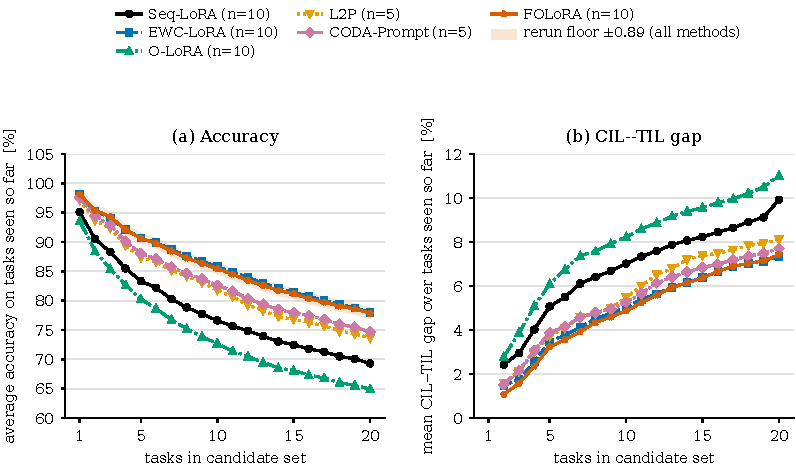
\includegraphics[width=0.92\linewidth]{figures/forgetting_curve_cifar100.pdf}
\caption{Average accuracy over the candidate classes seen so far (left) and the mean
CIL--TIL gap over those candidate sets (right) on Split CIFAR-100. Every point is a single
feature extraction of the \emph{terminal} model re-scored against a growing candidate set;
the horizontal axis is the number of tasks in that candidate set ($1$ to $20$, i.e.\ $5$ to
$100$ candidate classes at $5$ classes per task), not training time, so the leftmost point
already contains the forgetting incurred over the whole sequence. Each curve is drawn at the configuration \emph{and} the seed budget of its row in
Table~\ref{tab:main} --- ten seeds for Seq-LoRA, EWC-LoRA, O-LoRA and FOLoRA, five for L2P
and CODA-Prompt --- so its right-hand endpoint reproduces that row's
$\overline{\mathrm{ACC}}$. Six of the eight rows of Table~\ref{tab:main} are plotted;
InfLoRA and the SimpleCIL floor are tabulated but not drawn here, so the legend and the
table do not cover an identical row set. Those budgets differ between methods (Sec.~\ref{sec:setup}), so
the legend carries each curve's $n$ and the figure implies no equal $n$. No smoothing or
interpolation is applied --- the markers are the per-task measurements. The shaded band is
the run-to-run resolution of this measurement ($\pm0.89$ points, i.e.\ the standard deviation
of the difference between two independent runs of one configuration;
Sec.~\ref{sec:discussion}) --- a property of the protocol rather than of any one method, and
it applies to every curve shown. The vertical axis is bounded below at $60$, i.e.\ $4.94$
points under the lowest value plotted, rather than at zero; the full range is
$60$--$105$.}
\label{fig:curve-cifar}
\end{figure}

\begin{figure}[tbp]
\centering
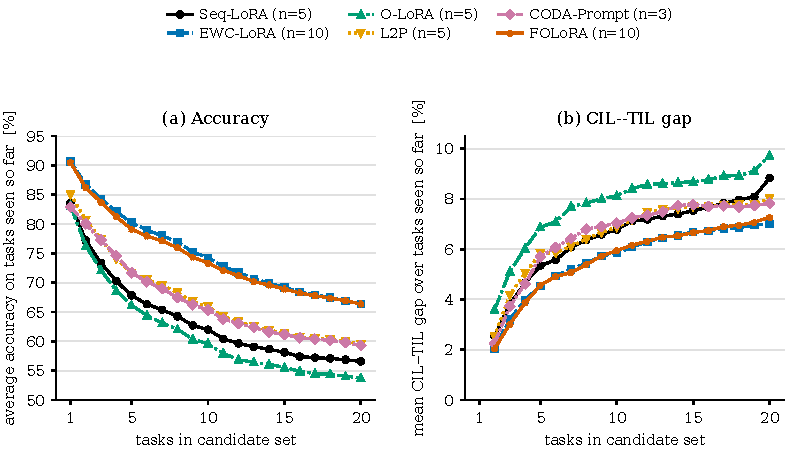
\includegraphics[width=\linewidth]{figures/forgetting_curve_imagenetr.pdf}
\caption{Average accuracy over the candidate classes seen so far (left) and the mean
CIL--TIL gap over those candidate sets (right) on Split ImageNet-R. As in
Fig.~\ref{fig:curve-cifar}, each point is a single feature extraction of the terminal model
re-scored against a growing candidate set --- the number of tasks in it, $1$ to $20$, i.e.\
$10$ to $200$ candidate classes at $10$ classes per task --- not a training trajectory. Each curve is drawn at the configuration \emph{and} the seed budget of
its row in Table~\ref{tab:main} --- CODA-Prompt on three seeds, L2P, O-LoRA and Seq-LoRA on
five, EWC-LoRA and FOLoRA on ten --- so its right-hand endpoint reproduces that row's
$\overline{\mathrm{ACC}}$. As in Fig.~\ref{fig:curve-cifar}, six of the eight rows of
Table~\ref{tab:main} are plotted; InfLoRA and the SimpleCIL floor are tabulated but not
drawn. Those budgets differ between methods (Sec.~\ref{sec:setup}), so
the legend carries each curve's $n$ and the figure implies no equal $n$. No
reproducibility-floor band is drawn, because that floor was measured on CIFAR-100 only and
we do not transfer it to another dataset. The vertical axis is bounded below at $50$, i.e.\
$3.72$ points under the lowest value plotted.}
\label{fig:curve-inr}
\end{figure}


% 两张图各占约半页，若不在此处冲刷，它们会漂到下一节中间，把 Appendix D 的正文劈成两段。
\clearpage

\section{Experimental environment}
\label{app:env}

All experiments reported here were run on one machine, so the wall-clock figures of
Table~\ref{tab:resources} are measured on the same device and under the same driver as each
other; they are relative costs between methods, not absolute budgets.
The GPU is an NVIDIA RTX 5060 Laptop with $8{,}151$\,MiB of memory (driver $592.01$) under
Windows~11, with Python $3.11.9$, PyTorch $2.11.0$ (CUDA $12.8$), torchvision $0.26.0$,
NumPy $2.4.6$, SciPy $1.17.1$ and scikit-learn $1.9.0$. Training is single-process, without
data-parallel or mixed-precision accumulation.
The backbone is the torchvision ViT-B/16 pre-trained on ImageNet-1k
(\texttt{IMAGENET\_1K\_V1}), used frozen except where a baseline trains the backbone by
construction. Both benchmarks are resized to $224\times224$ and normalised with the ImageNet
statistics; the training pipeline adds a random horizontal flip, the test pipeline does not.
CIFAR-100 is split into $20$ tasks of five classes and ImageNet-R into $20$ tasks of ten
classes, with the class orders fixed by the seed reported alongside each result; every run
writes its full configuration to a \texttt{config.json} in its own directory, so any number
in this paper can be traced to the configuration that produced it.
Each reported mean and standard deviation is over the seeds listed where the number is used;
single-run figures are labelled as such.
